\documentclass[aspectratio=169]{beamer}
\usetheme{Boadilla}
\usepackage{tikz}
\usetikzlibrary{positioning, arrows.meta, shapes.geometric, calc}

\title{Kaggle Bot Architecture}
\subtitle{Simulate10Next}
\author{Handover Presentation}
\date{\today}

\begin{document}

\frame{\titlepage}

% --- SLIDE 1 ---
\begin{frame}
    \frametitle{High-Level Philosophy}
    \begin{itemize}
        \item \textbf{Data-Driven Design:} The bot handles the game state as Pandas DataFrames.
        \item \textbf{Vectorized Operations:}
        \begin{itemize}
            \item Relies on DataFrame transformations rather than iterative loops for speed.
            \item Converting to Polars Lazy would make it even faster.
        \end{itemize}
    \end{itemize}

    \vspace{0.4cm}
    \begin{block}{Presentation Overview}
        \begin{tabular}{cl}
            \textbf{Slide 3} & The Architecture (\texttt{GameConfig}, \texttt{PhysicsEngine}, \texttt{StrategyPipeline}, \texttt{agent()}) \\[2pt]
            \textbf{Slide 4} & The \texttt{StrategyPipeline} --- four-stage data pipeline \\[2pt]
            \textbf{Slide 5} & Short-Term Roadmap --- Supply Chains \& Kinematic Profiles \\[2pt]
            \textbf{Slide 6} & Long-Term Roadmap --- Simulate10NextAction \\
        \end{tabular}
    \end{block}
\end{frame}

% --- SLIDE 2 ---
\begin{frame}
    \frametitle{The Architecture}
    \centering
    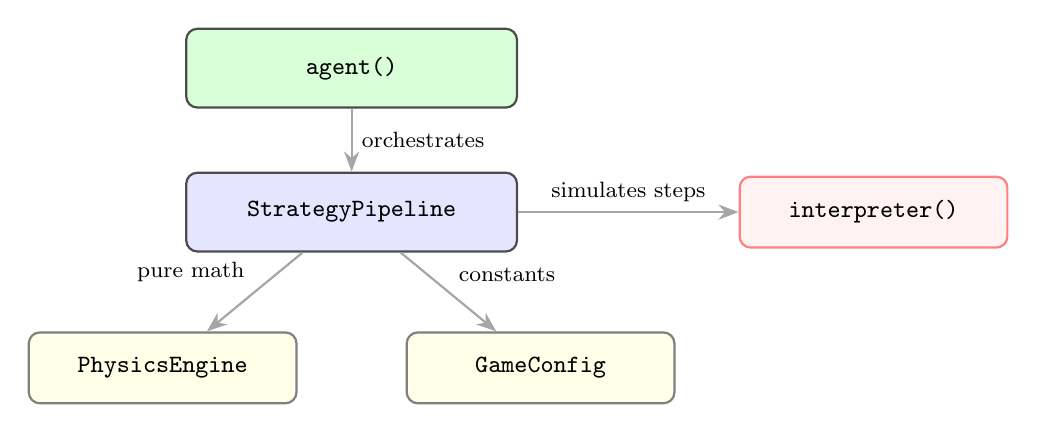
\begin{tikzpicture}[
        box/.style={rectangle, draw=black!70, thick, fill=blue!10, rounded corners,
                    minimum width=4.2cm, minimum height=1cm, align=center, font=\small},
        sbox/.style={rectangle, draw=black!50, thick, fill=yellow!10, rounded corners,
                     minimum width=3.4cm, minimum height=0.9cm, align=center, font=\small},
        ibox/.style={rectangle, draw=red!50, thick, fill=red!5, rounded corners,
                     minimum width=3.4cm, minimum height=0.9cm, align=center, font=\small},
        arrow/.style={-{Stealth[scale=1.1]}, thick, draw=gray!70}
    ]
        \node[box, fill=green!15] (agent) {\textbf{\texttt{agent()}}};
        \node[box, below=0.8cm of agent] (pipeline) {\textbf{\texttt{StrategyPipeline}}};
        \node[ibox, right=2.8cm of pipeline] (interp) {\textbf{\texttt{interpreter()}}};
        \node[sbox, below=1.0cm of pipeline, xshift=-2.4cm] (physics) {\textbf{\texttt{PhysicsEngine}}};
        \node[sbox, below=1.0cm of pipeline, xshift= 2.4cm] (config)  {\textbf{\texttt{GameConfig}}};

        \draw[arrow] (agent)    -- node[right, font=\footnotesize] {orchestrates} (pipeline);
        \draw[arrow] (pipeline) -- node[above, font=\footnotesize] {simulates steps} (interp);
        \draw[arrow] (pipeline) -- node[above left,  font=\footnotesize] {pure math}  (physics);
        \draw[arrow] (pipeline) -- node[above right, font=\footnotesize] {constants}  (config);
    \end{tikzpicture}

    \vspace{0.4cm}
    \begin{itemize}
        \item \textbf{\texttt{agent()}} manages Kaggle I/O and global state (\texttt{step}, \texttt{player\_id}).
        \item \textbf{\texttt{StrategyPipeline}} transforms each observation into moves via four sequential stages.
        \item \textbf{\texttt{interpreter()}} is the Kaggle game engine --- called by \texttt{\_01} to simulate 10 steps forward.
        \item \textbf{\texttt{PhysicsEngine}} and \textbf{\texttt{GameConfig}} are stateless and never modified.
    \end{itemize}
\end{frame}

% --- SLIDE 3 ---
\begin{frame}
    \frametitle{The Pipeline Workflow}
    \begin{columns}[T]
        \begin{column}{0.35\textwidth}
            \centering
            \vspace{0.15cm}
            \scalebox{0.99}{%
            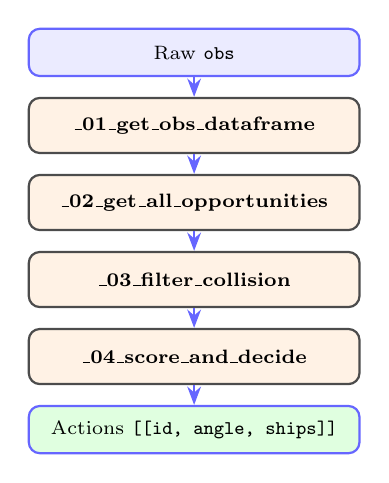
\begin{tikzpicture}[
                node distance=0.25cm,
                process/.style={rectangle, draw=black!70, thick, fill=orange!10, rounded corners,
                                minimum width=4.2cm, minimum height=0.7cm, align=center, font=\scriptsize},
                io/.style={rectangle, draw=blue!60, thick, fill=blue!8, rounded corners,
                            minimum width=4.2cm, minimum height=0.6cm, align=center, font=\scriptsize},
                arrow/.style={-{Stealth}, thick, draw=blue!60}
            ]
                \node[io] (raw) {Raw \texttt{obs}};
                \node[process, below=of raw] (p1) {\textbf{\_01\_get\_obs\_dataframe}};
                \node[process, below=of p1]  (p2) {\textbf{\_02\_get\_all\_opportunities}};
                \node[process, below=of p2]  (p3) {\textbf{\_03\_filter\_collision}};
                \node[process, below=of p3]  (p4) {\textbf{\_04\_score\_and\_decide}};
                \node[io, fill=green!12, below=of p4] (out) {Actions \texttt{[[id, angle, ships]]}};

                \draw[arrow] (raw) -- (p1);
                \draw[arrow] (p1)  -- (p2);
                \draw[arrow] (p2)  -- (p3);
                \draw[arrow] (p3)  -- (p4);
                \draw[arrow] (p4)  -- (out);
            \end{tikzpicture}}
        \end{column}
        \begin{column}{0.65\textwidth}
            \small
            \begin{itemize}
                \item \textbf{\_01:} Simulates 10 future steps via \texttt{interpreter()}.
                \begin{itemize}
                    \item Outputs \texttt{df\_s} (planet states) and \texttt{planet\_disp}.
                    \item Labels each planet as \texttt{fix}, \texttt{moving}, or \texttt{comet}.
                \end{itemize}
                \item \textbf{\_02:} Cross-joins sources $\times$ targets across all steps.
                \begin{itemize}
                    \item Swept-pair collision finds valid intercept trajectories.
                    \item Outputs \texttt{pa} (Possible Attacks) with angle cones.
                \end{itemize}
                \item \textbf{\_03:} Removes occluded trajectories.
                \begin{itemize}
                    \item Drops any path blocked in the same angular cone by an earlier target.
                \end{itemize}
                \item \textbf{\_04:} Scores and selects one move per source.
                \begin{itemize}
                    \item Ranks by time-cost-adjusted production value.
                \end{itemize}
            \end{itemize}
        \end{column}
    \end{columns}
\end{frame}

% --- SLIDE 4 ---
\begin{frame}
    \frametitle{Roadmap: Enhancing \texttt{\_04\_score\_and\_decide}}
    \begin{block}{1. Role-Based Planet Logic (Supply Chains)}
        \begin{itemize}
            \item \textbf{Conquerors} --- Planets with $\ge 1$ enemy within their 5 nearest neighbors.
            \begin{itemize}
                \item Prioritized for frontline attacks.
            \end{itemize}
            \item \textbf{Suppliers} --- Planets where all 5 nearest neighbors are friendly.
            \begin{itemize}
                \item Prioritized to send reinforcements to Conquerors.
            \end{itemize}
        \end{itemize}
    \end{block}

    \begin{block}{2. Kinematic Targeting Profiles}
        \begin{itemize}
            \item Scoring differentiates by motion-type pair (source $\times$ target):
                  \texttt{fix}, \texttt{moving}, or \texttt{comet}.
            \item Moving targets are preferred --- they allow attacking planets on the far side
                  of the board by intercepting their orbit.
        \end{itemize}
    \end{block}
\end{frame}

% --- SLIDE 5 ---
\begin{frame}
    \frametitle{Long-Term Roadmap: Simulate10NextAction}
    \begin{block}{Compute Caching (Beating the Time Limit)}
        \begin{itemize}
            \item Pre-compute 500-step positions for all planets at $T=0$.
            \item Cache Fix $\rightarrow$ Fix opportunities globally --- geometry never changes.
            \item Cache Moving $\rightarrow$ Moving matrices; adapt each turn by rotating angles
                  by $\omega \times \Delta t$.
            \item Track spawned fleets immediately --- compute destination once, reuse every step.
            \item With caching in place: simulate all candidate actions 10 steps forward
                  and select the subset that maximises the board score.
        \end{itemize}
    \end{block}
\end{frame}

\end{document}
